\section{Verhaltensformular}
\label{sec:verhaltensformular}

Damit die Videos ausgewertet werden können, wurde ein Verhaltensformular erstellt. Dieses Formular lehnt sich an generelle Ausdrucksweisen von Babies an.
Die Auswertung kann in späteren Projekten ausgeführt werden.\\

Das Formular wird auf der Webapplikation unterhalb des Videos eingeblendet und enthält die wichtigsten Merkmale. Diese Anzeichen können durch den ganzen Körper oder durch konkrete Bewegungen ersichtlich sein. Daher sind als \dq wichtigste Merkmale \dq das Gesamtverhalten \dq ruhig \dq und \dq unruhig \dq ausgewählt. Falls das nicht zutrifft, kann man in das darunter liegende Textfeld das Gesamtverhalten des Babies eingetragen werden.

\begin{figure}[]
	\centering
		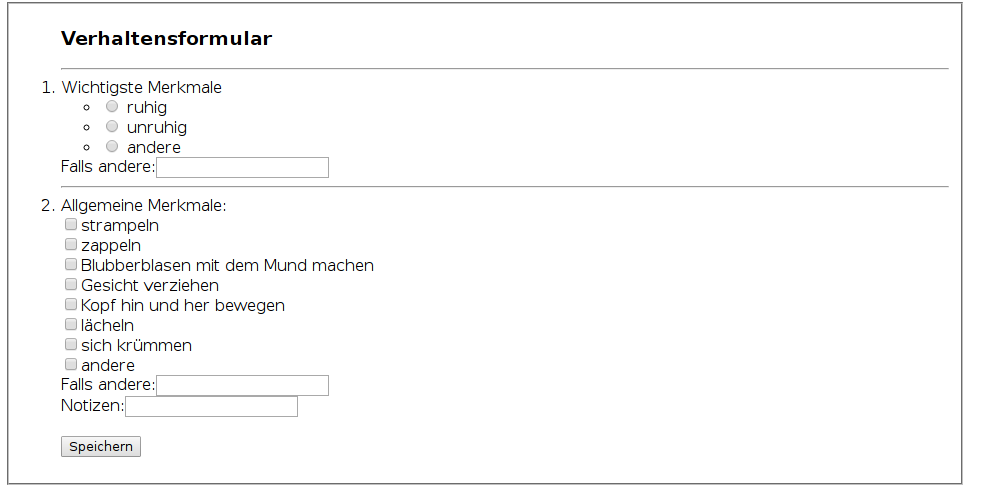
\includegraphics[width=0.8\textwidth]{includes/evalsys/graphics/verhaltensformular}
	\caption{Verhaltensformular zur analyse des Verhaltens des Babies}
	\label{fig:verhaltensformular}
\end{figure}

Um die Anzeichen genauer zu spezifizieren, sind weitere Eigenschaften aufgeführt, die ohne Ton erkannt werden können. Diese können aus der Abbildung \ref{fig:verhaltensformular} entnommen werden.\\
Um die eingegebenen Daten auf dem Server zu speichern, wurde ein Speicherknopf implementiert. Das Auslesen und Speichern der Daten des Formulars funktioniert mittels der POST-Methode. Diese greift auf den aktuellen Zustand der angegebenen Textfelder, Radiobuttons und Checkbuttons zu.
